\chapter{Introduction}
\label{ch:introduction}
	Forest covers approximately 30\% of the global land surface, while roughly 50\% of the global forest area can be attributed to tropical forests \citep{WWF2016}. The tropical tree cover envelop the global land surface between 23$^\circ$ north (the tropic of Cancer) and 23$^\circ$ south (the tropic of Capricorn) as figure \ref{fig:tropicalzone} shows. Tropical forest ecosystems are a pivotal component of the earth system. They are crucial factors for climate, water cycle, soil health, biodiversity, and source of natural goods for human subsistence. These forests are major contributor to the global carbon and energy cycle and house roughly 50\% of the species and two thirds of all plant species \citep{Wright2005,Jordan2005}. Further, it is assumed that tropical forests have a major impact on the hydrologic regime. In developing tropical countries like Cambodia or Myanmar timber extraction and trade is important part of the economy, while fuelwood accounts for approximately 30\% of the total primary energy supply in developing countries over the tropics \citep{Jordan2005}. However, this globally unique ecosystem and its diverse functions is endangered by several causes \citep{WWF2016}.
	\begin{figure}[ht]
		\centering
		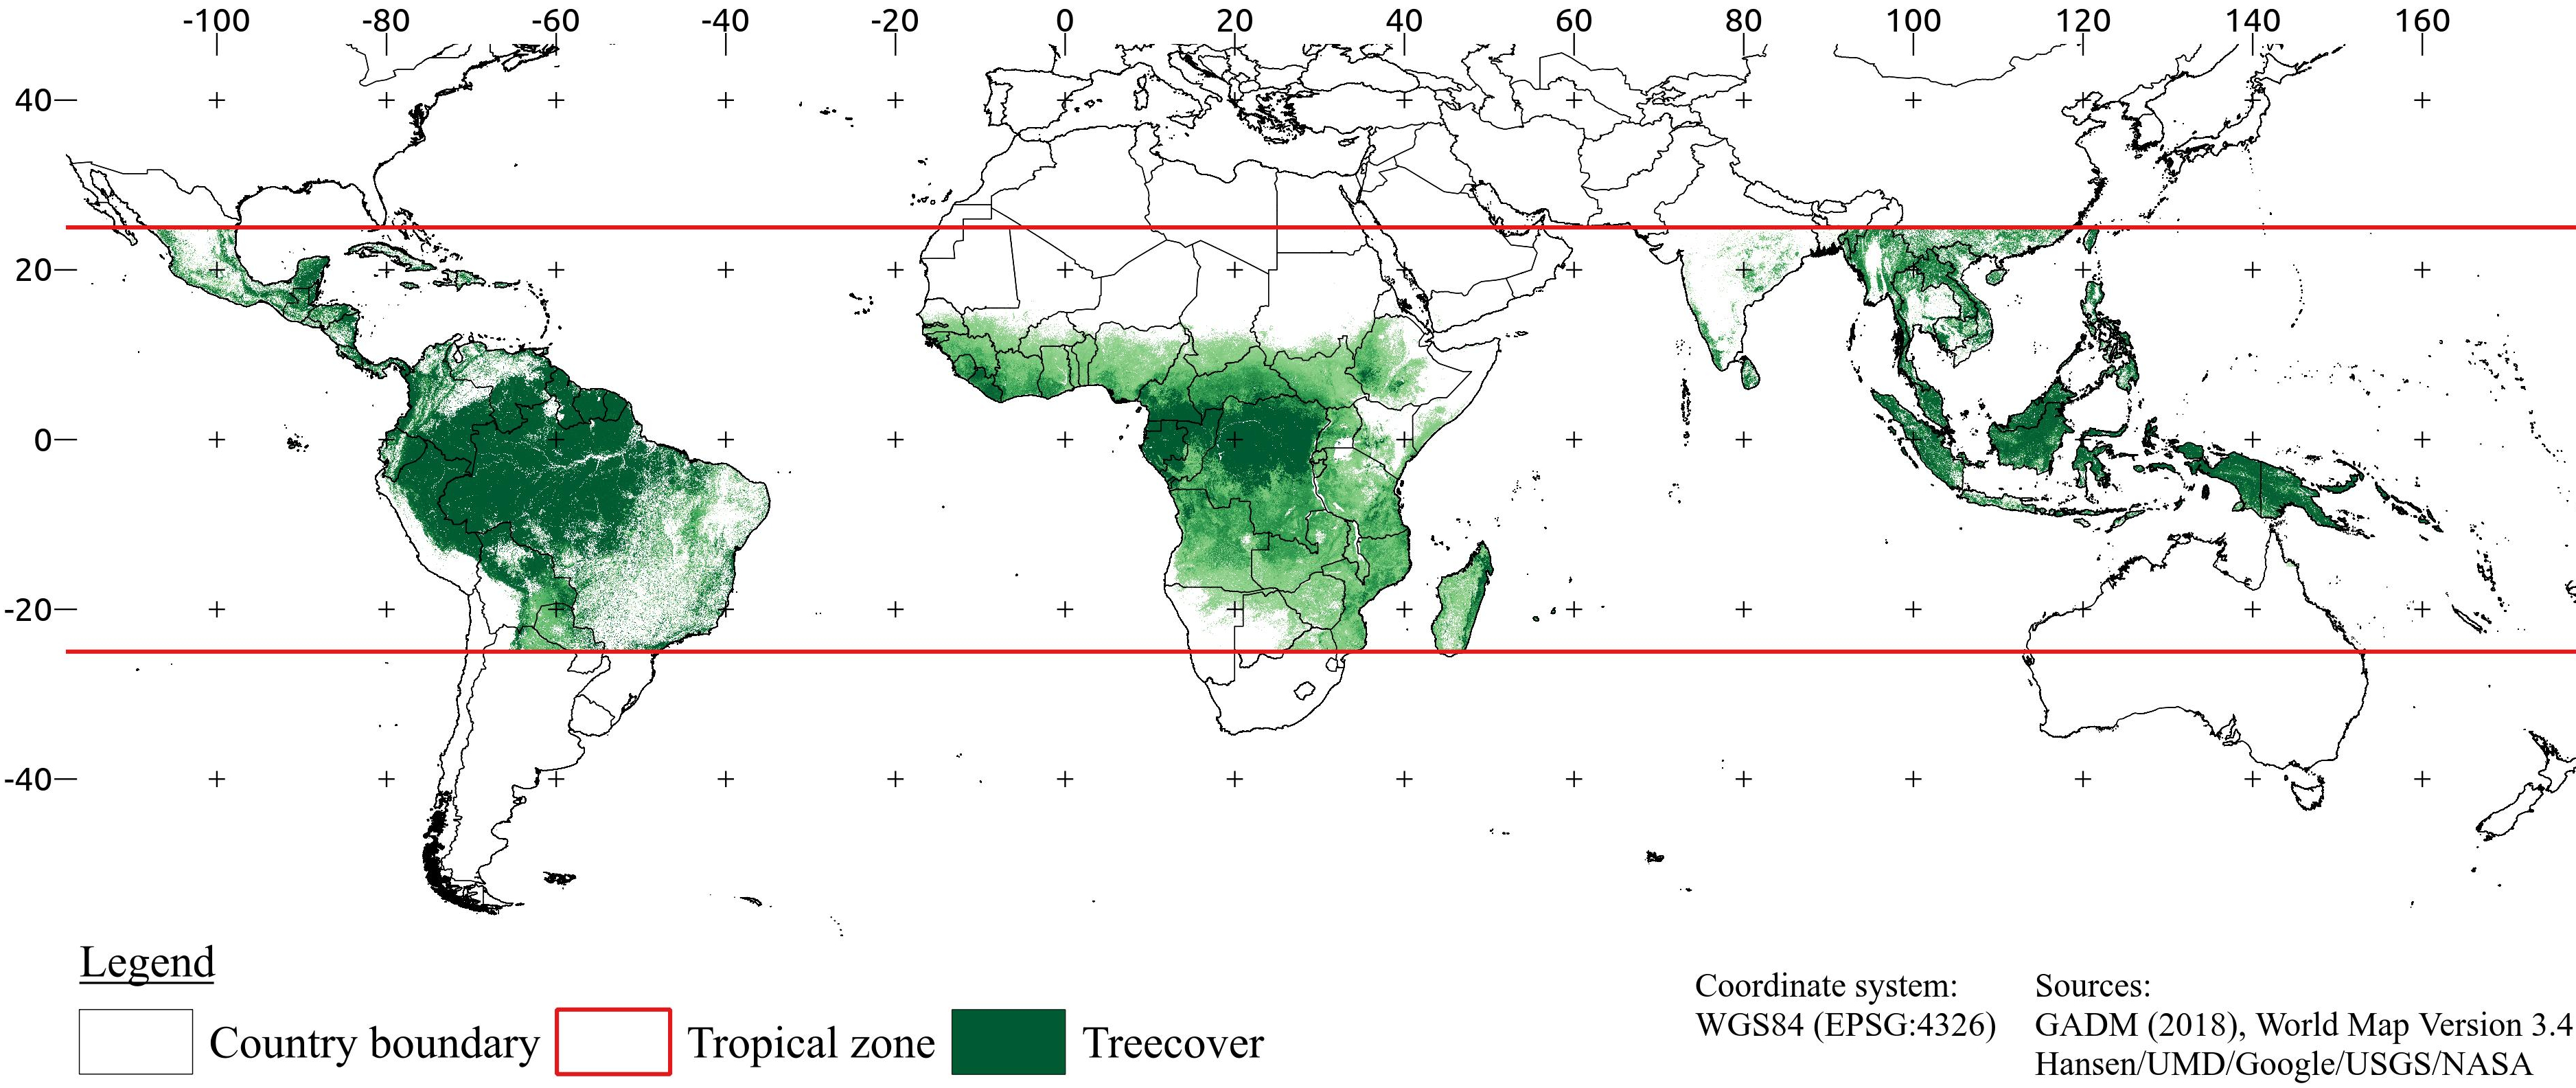
\includegraphics[scale=.97]{img/intro_overview_frameless}
		\caption[Tropical zone and forest]{\textbf{Tropical zone and forest}}
		\label{fig:tropicalzone}
	\end{figure}

	Since the 1990s approximately 3.1\% of the global forest area is lost due to deforestation, while approximately 35\% of the tree cover loss is within the tropical zone \citep{FAO2016}. Between 1990 and 2015 the top ten countries of highest annul net loss of forest are concentrated in the tropical belt, which highlights the severe forest alterations within this zone \citep{FAO2010,FAO2016}. Forest loss or deforestation is defined as the removal of trees or forest stands from land surface area, which is then transformed to other LULC (Land use/Land cover) types. Deforestation and LULC change is one of the major causes for the fragmentation of the tropical forest cover \citep{Taubert2018}. Further, tree cover loss is a dominant cause for the emission of \ac{GHG} \citep{Don2010,Baccini2012}. Additionally, the continues process of deforestation jeopardizes the carbon fixing capacity of tropical forest \citep{Baccini2017}. Thus it is important to scrutinize the causes of deforestation. \citet{Geist2001} introduced the conceptual framework of proximate, underlying, and other causes of tropical deforestation to group the driving forces of forest cover change. The term \ac{PDD} or direct deforestation driver encompass anthropogenic actions that change forest to other \ac{LC} types. Whereas, the new \ac{LC} type is considered as the direct deforestation driver. Proximate causes of deforestation are subdivided into three different categories: agricultural expansion, wood extraction, and infrastructure expansion. Examples for deforestation driven by agriculture are the expansion of pastures, cropland, and tree crops as exemplified in the figure \ref{fig:deforestationexamples}. Whereas, the other two categories, wood extraction and infrastructure expansion encompass the following causes: fuelwood extraction, charcoal production, transport infrastructure, and settlement expansion. The term underlying causes refers to complex social, political, economic, technological, and cultural interactions, which underpin the \acp{PDD}. The category of other causes for deforestation comprises land characteristics, biophysical drivers, and social trigger events. Features of land characteristics are the soil quality and landscape topography, which could determine the shape and extent of anthropogenic deforestation actions. Only a few countries survey \acp{PDD} by a systematic procedure and spatial details are even more rare \citep{Sy2015,Hosonuma2012}. Whereby, the availability of spatial explicit data of \acp{PDD} is important because this data can be used to derive other features to describe deforestation comprehensively \citep{Hosonuma2012}. The advances in the field of remote sensing and the availability of country meta-data has fostered the research on \acp{PDD} on a continental or regional scale (e.g. \citet{Sy2015,Austin2019,Zalles2018,Meyfroidt2013,Caldas2013,Graesser2015,Ruf2014,Connette2016,Barima2016,Furumo2017,Vijay2018}). Although, the availability of global scaled data on direct deforestation driver is still limited (e.g. \citet{Curtis2018,Hosonuma2012,Geist2002,DeFries2010,Carter2018}). Further, only one study scrutinized the disposition of \acp{PDD} in a spatial explicit procedure on a global range (e.g. \citet{Curtis2018}). All the beforehand mentioned studies agree on the fact, that agricultural expansion dominates the the tree cover loss as \ac{PDD}. Whereby, each study estimates a varying size for agricultural causes and other causes, which could be related to differences in the methodology. Some studies relay on meta-analysis or country meta-data and use an empirical approach to predict \acp{PDD} (e.g. \citet{Hosonuma2012,Geist2002,DeFries2010,Carter2018,Ruf2014}), while other studies apply sample-based methods in combination with statistical models and visual interpretation of remotely sensed data (e.g. \citet{Sy2015,Austin2019,Curtis2018,Meyfroidt2013,Caldas2013}). Additionally, some studies relay only on remote sensing of the environment to predict the proximate causes of deforestation (e.g. \citet{Caldas2013,Zalles2018,Graesser2015,Connette2016,Barima2016}). On the fact that these studies need a vast amount of expert knowledge and in some cases repetition of time consuming processes they require a large effort for repetition. Further, the studies that estimate the \acp{PDD} spatially explicit are only in low resolution available, which overlooks small-holder deforestation \citep{Curtis2018,Caldas2013}. Additionally, all studies more or less present the proximate causes on deforestation already as aggregates of the three groups \citet{Geist2001} suggest. Therefore, it is not possible to derive regional or continental differences between the patterns of cropland and pasture expansion.
	\begin{figure}[ht]
		\centering
		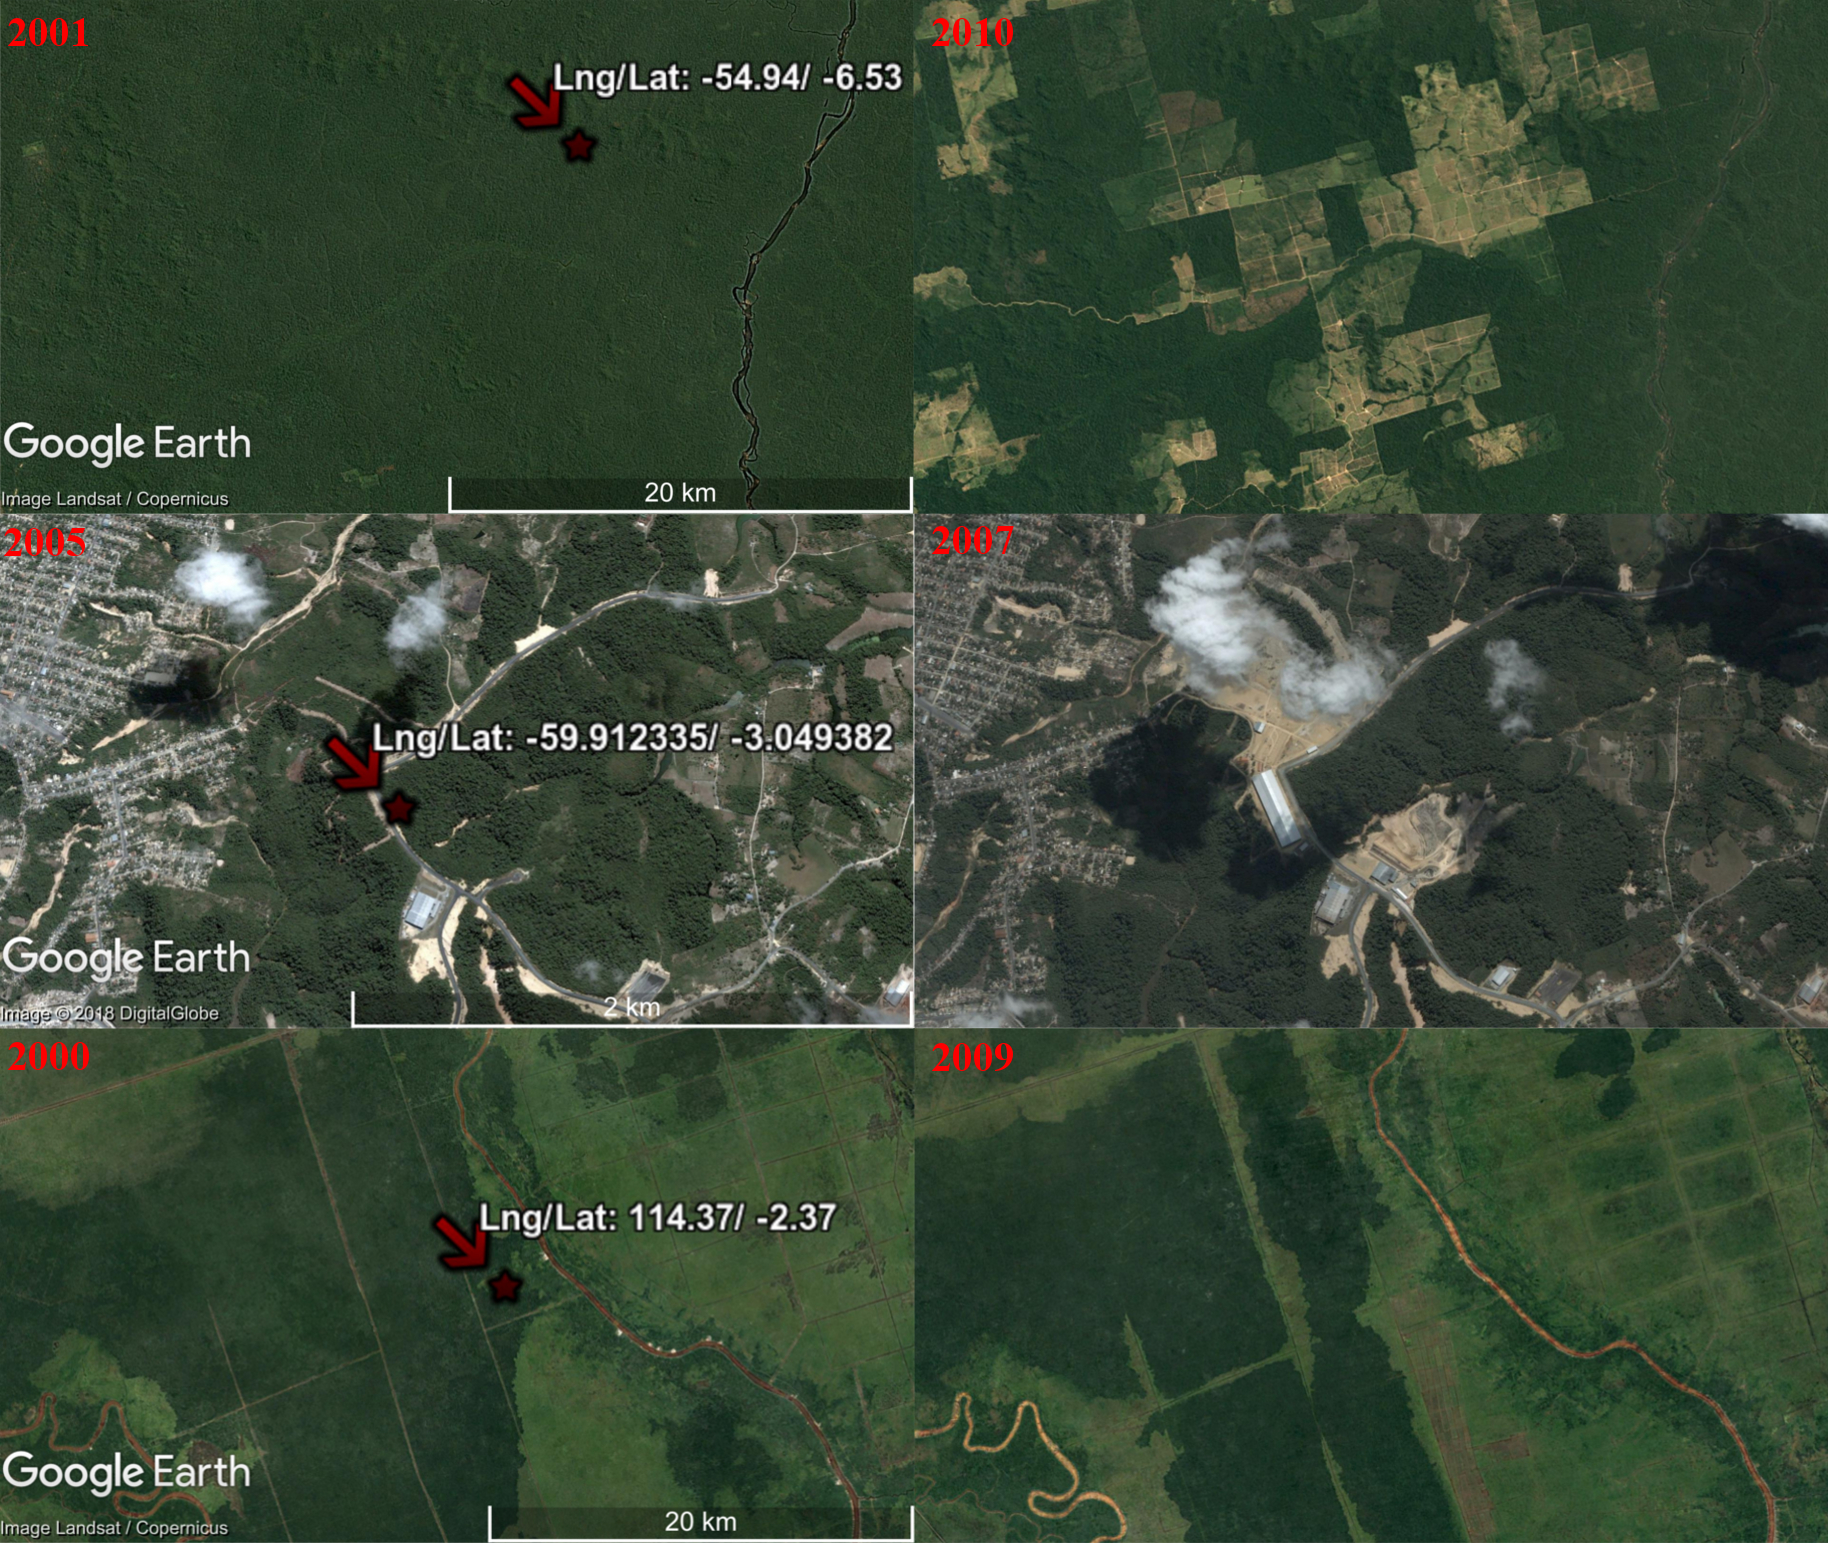
\includegraphics[scale=0.53]{img/deforestation_examples}
		\caption[Examples of proximate deforestation drivers]{\textbf{Examples of proximate deforestation drivers:} The transformation of forests by the expansion of pastures in the Brazilian province of Pará (top), the expansion of settlements in the Brazilian province of Amazonas (center), and the expansion of tree crops (oil palm) in the Indonesian province of Central Kalimantan (bottom).}
		\label{fig:deforestationexamples}
	\end{figure}

	The \ac{LC} conversion of tropical forests induced by \acp{PDD} are the second largest source of anthropogenic-induced \ac{GHG} emissions \citep{Don2010}. The main \ac{GHG} released by deforestation to the atmosphere is carbon, which is a major contributor to climate change. Therefore, avoided tropical deforestation could be a significant contribution to climate change mitigation \citep{Don2010}. Further, the United Nations (UN) initiative on Reducing Emissions from Deforestation and Degeneration (REDD+) presents valuable incentives for developing sub-tropical and tropical countries to reduce their emissions from forests \citep{Avitabile2016}. Therefore, carbon emission accounting has a key role to implement REDD+ activities. The total emissions arising from deforestation can be broken down into many different categories, e.g. \ac{GHG} emissions from biomass removal, emissions resulting from \ac{SOC} dynamics, \ac{GHG} emissions arising from the resulting \ac{LU} activity \citep{Avitabile2016}. Carbon emissions from biomass removal arise from aboveground and below-ground biomass of woody vegetation. The quantity of theses emissions is determined by two factors: (1) the rate of deforestation, and (2) the biomass density of the former tree covered area \citep{Houghton2012a}. Carbon loss from \ac{SOC} changes are controlled by two key factors: (1) the decomposition rate of \ac{SOC} controlled by the surrounding micro-climate, and (2) variations in the quality and quantity of carbon cycled through the soil system \citep{Don2010}. Deforestation alters both factors and the subsequent \ac{LC} transition controls the soil erosion, which may be is a major pathway of \ac{SOC} loss. Tropical soils are a major carbon storage, which account for 30\%-60\% of the carbon stored in forests \citep{Don2010}. Further, tropical vegetation are estimated to store approximately 228.7 Gt C \citep{Baccini2012}. Therefore, it is of outstanding importance to quantify carbon losses by biomass removal and \ac{SOC} change. Studies that estimate the carbon losses by biomass removal on a global or regional scale are common in science, while the assessments range between 600-1400 Mt C yr$^{-1}$ for 2000-2010 (e.g \citet{Houghton2012,Achard2014,Sy2015,Baccini2012}). Further, several studies scrutinized the impact of different \ac{LC} transition types on \ac{SOC} in terms of carbon losses (e.g. \citet{Don2010,Rahman2018,Villarino2017}). However, no study linked these \ac{SOC} change coefficients to tropical forest \ac{LC} transitions by \acp{PDD} to quantify the total carbon losses. Further, it is unknown at which magnitude the \ac{SOC} emissions contribute to the carbon losses by biomass removal.

	Tropical ecosystems have a crucial impact on the well-being and subsistence of current and future generation out of humanity through the provision of regulatory, supporting, provisioning, and cultural services \citep{Costanza1997}. On the fact that deforestation and \ac{LC} changes lead to major changes in ecosystem services by altering the shape of forest biomes it is crucial to evaluate these impacts not only in terms of \ac{GHG} emissions but also for key ecosystem services as water, regulation, biodiversity etc. For the quantification of these ecosystem services a economic process is applied to assess the monetary value of each service per ecosystem. These \acp{ESV} can be a strong tool to determine the impact of certain management practices on ecosystem structures and raise the public awareness that ecosystems are scarce resources which could not be treated as free inexhaustible goods \citep{Groot2012}. The monetary valuation of ecosystems should be not understand as privatizing or commodifying them as tradeable goods for private markets \citep{Costanza2014,Song2018}. Further, the valuation of ecosystem services has fostered natural capital accounting and inclusion in national policies \citep{Song2018}. During the past decade scientific research fostered the development of several valuation approaches like direct market valuation, revealed preference, stated preference and benefit transfer \citep{Song2018}. Benefit transfer is the conceptually simplest approach to estimate the \ac{ESV}, but is widely used especially for estimates over large geographic regions \citep{Costanza1997,Song2018,Costanza2014}. This approach uses a constant unit value per hectare of ecosystem type and multiplies that value by the area of each type to obtain the aggregated total \citep{Costanza2014}. Remotely sensed land cover dataset are widely applied in the estimation \acp{ESV} to derive a global valuation of ecosystems by applying \ac{ESV} unit values \citep{Song2018}. The literature provides several studies on ecosystems and its monetary values. However, the by far most used global unit values for ecosystems are prepared by \citet{Costanza2014}. This values are applied in several studies (e.g. \citet{Costanza2014,Song2018,Sannigrahi2018,Kreuter2001,Wang2006,Zhao2004}). \citet{Siikamaki2015} introduced recently global and regional \ac{ESV} unit values for forest ecosystems. These values are used by the World Bank in its wealth program on developing country-level indicators of sustainability \citep{Siikamaki2015}. Another well known datasets of \acp{ESV} is provided by \citet{Groot2012}. Till now several studies estimated \ac{ESV} dynamics at local or regional scales (e.g. \citet{Kreuter2001,Wang2006,Zhao2004}). Global-scale studies that estimate the monetary value of our planetary ecosystems and the losses by \ac{LC} change are relatively rare (e.g. \citet{Costanza1997,Costanza2014,Sannigrahi2018,Song2018}). The ecosystem estimates of this global studies ranging between 49.4-75.1 trillion dollar per year, while losses due to \ac{LC} change ranging between 1.21-20.2 trillion dollar per year, all values in 2007 Int'I\$ y$^{-1}$. The \ac{ESV} loss due to tropical deforestation ranges between 550.7 billion and 3.5 trillion dollar per year. These estimates are derived from \ac{LC} data at a coarse spatial resolution between 1 km and 300 m except the estimates of \citet{Song2018}, that are derived from the \ac{GFC} dataset at spatial resolution of 30 m. However, the \ac{ESV} accounting of \citet{Song2018} lacks of an importing filtering of the \ac{GFC} data and it does not consider \ac{ESV} dynamics from \ac{LC} change. To best of our knowledge no study accounted the \ac{ESV} dynamics in regards of \ac{ESV} loss, gain and balance exclusively for tropical forest loss and its \acp{PDD} by using high resolution data.

	\section{Research objectives}
		Based on the research gaps we want to focus on the following research questions to analyze tropical deforestation for the 2001-2010 time period:
		\begin{itemize}
			\item What are the proximate drivers of tropical deforestation?
			\item What quantity have the gross carbon loss by removal of biomass and soil organic carbon change?
			\item What are the magnitudes of the ecosystem service value dynamics?
		\end{itemize}

